\documentclass[9pt,twocolumn,twoside]{styles/osajnl}
\usepackage{fancyvrb}
\usepackage{url}
\journal{i524} 

\title{Google Bigtable}

\author[1,*]{Mark McCombe}

\affil[1]{School of Informatics and Computing, Bloomington, IN 47408, U.S.A.}

\affil[*]{Corresponding authors: mmccombe@iu.edu}

\dates{paper1, \today}

\ociscodes{Bigtable, Google, NoSQL, I524}

% replace this with your url in github/gitlab
\doi{\url{https://github.com/cloudmesh/sp17-i524/tree/master/paper1/S17-IO-3012/report.pdf}}


\begin{abstract}

Google's NoSQL database, Bigtable, is a critical technology in big data for its use internally at Google, as the external service Cloud Bigtable, and for inspiring open source technologies such as Hbase.  An overview of Bigtable's storage model and architecture are presented, including available APIs, shell access, and the graphical user interfaces. Performance and security features of Bigtable are discussed along with technologies related to Bigtable. Internal and external use cases involving Bigtable are detailed. Finally, educational resources for learning more about Bigtable are listed.
\newline
\end{abstract}

\setboolean{displaycopyright}{true}

\begin{document}

\maketitle

\section{Introduction}

Google Bigtable is a NoSQL database developed by Google, built on several Google technologies, including Google File System, Chubby Lock Service, and SSTable\cite{www-wikibigtable}.  One of the earliest NoSQL databases, development on Bigtable started in 2004 and Bigtable was introduced to the public in a paper published in 2006 \cite{introbigtable}. Bigtable is important to Big Data both for its use internally at Google and externally as Cloud Bigtable, which was made available in May 2015. Google uses Bigtable to power many core Google products, such as Search, Analytics, Maps, Earth, Gmail, and YouTube. \cite{www-wikibigtable}.

Bigtable has inspired other technologies, notably Hbase \cite{www-hbase} an open source distributed, scalable database that was modeled after Bigtable and is typically used along with Hadoop and Hadoop Distributed File System (HDFS) as part of the Apache Big Data Stack.

While Bigtable is a significant technology in Big Data due to its use in Google products and role in the development of other NoSQL technologies, Cloud Bigtable itself is not one of the more popular databases available today.  DBEngines ranks Cloud Bigtable only 6 of 9 among Wide Data Stores and 166 of 285 among databases overall for popularity \cite{www-dbengines}.

\section{Storage Model}

Bigtable stores data in tables, which are sorted by key/value maps. Tables have rows, typically a single entity, and columns which contain values for the rows. Rows are index by a row key. Columns have both a family and a qualifier, which is unique within a family \cite{www-bigtabledocoverview}.

Figure 1 shows the Bigtable Storage model. It contains four rows (row keys - gwashington, jadams, tjefferson, and wmckinley), one column family (follows), and four column identifiers (also gwashington, jadams, tjefferson, and wmckinley). Tables in Bigtable are sparse, meaning that a cell will not take up space if it does not contain data (as in the case of jadams/wmckinley).  Intersections may contain multiple cells with different timestamps (as in the case of tjefferson/gwashington and jadams/tjefferson) providing a historical record of data in Bigtable \cite{www-bigtabledocoverview}.

\begin{figure}[ht]
  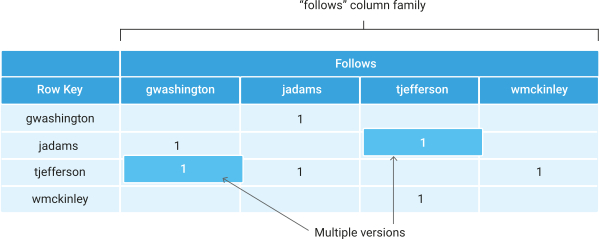
\includegraphics[scale=0.45]{images/bigtable-example.jpg}
  \caption{Bigtable Data Model}\cite{www-bigtabledocoverview}
\end{figure}

\section{Architecture}

The architecture of Cloud Bigtable is depicted in Figure 2.  As shown, client requests come through a front-end server pool and are directed to a Bigtable node (called tablet servers when Bigtable was introduced in 2006). Bigtable nodes are organized into Bigtable clusters, which in turn each belong to a Bigtable instance \cite{www-bigtabledocoverview}.

Tables in Bigtable are sharded tablets, which contain blocks of contiguous rows, to balance query workload. Tablets are stored in SSTable format, which provides a map from keys to values, in Google's file system Colossus and housed in Google's data centers. Each tablet belongs to a specific node \cite{www-bigtabledocoverview}.

The approach of storing data in tablets rather than rows provides performance benefits and fault tolerance to Bigtable. Because no data needs to be copied, rebalancing tablets between nodes is fast. If a Bigtable node fails, no data is lost and recovery is quick because only metadata needs to be copied to the new node  \cite{www-bigtabledocoverview}.

Bigtable balances data volume and workload across clusters automatically. Bigtable handles this automatically, reducing the administrative effort required\cite{www-bigtabledocoverview}.


\vspace{-\topsep}


\begin{figure}[ht]
  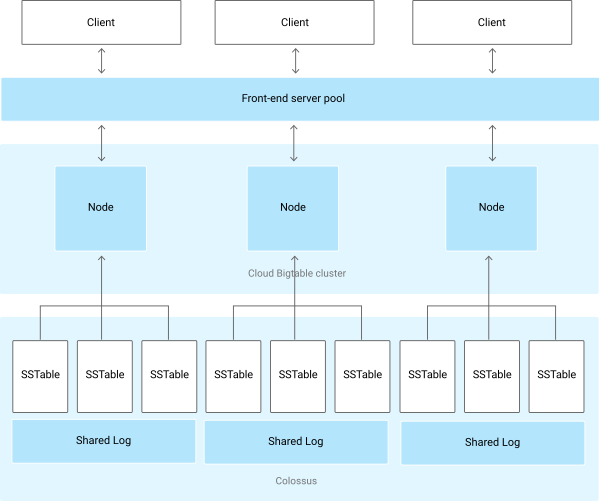
\includegraphics[scale=0.45]{images/bigtable-architecture.jpg}
  \caption{Bigtable Architecture} \cite{www-bigtabledocoverview}
\end{figure}

\subsection{API}

Bigtable APIs exist for several languages \cite{www-bigtabledocapi}.

\vspace{-\topsep}
\begin{itemize}
\item HBase Client for Java
\item Go Client
\item Python Client
\item Bigtable-dotnet (.NET)
\item Scio (Scala)
\item Dataflow Connector (for use in Pipelines)
\end{itemize}

Bigtable can also integrate with Google Cloud Dataflow, a cloud based, big data programming model, and with Apache Hadoop through the use of Google Cloud Dataproc \cite{www-bigtabledocapi}.

\subsection{Shell Access}


Shell access in Cloud Bigtable can be performed through the HBase Shell \cite{www-hbaseshell}. The HBase shell provides a Ruby environment that allows functions in BigTable to be executed on the command line and provides scripting capabilities. HBase shell commands fall into four main categories \cite{www-hbaseshell2}.

\vspace{-\topsep}
\begin{itemize}
\item General Commands - version, status, etc.
\item Table Management Commands - create, drop, alter, etc.
\item Data Manipulation Commands - count, get, delete, etc.
\item Cluster Replication Commands - start/stop replication, add/remove peer 
\end{itemize}
\vspace{-\topsep}

In addition to HBase Shell, cbt, a command line tool written in Go, can be used to perform operations against Bigtable \cite{www-cbt}. 


\subsection{Graphical Interface}

BigQuery Web UI is a graphical interface, designed to run in Google's Chrome browser, that allows users to interact with BigTable in various ways \cite{www-bigquerywebui}.

\vspace{-\topsep}
\begin{itemize}
\item Load and Export Data
\item Run Queries
\item Create, Delete, Copy, and Append to Tables 
\item View, Add, Delete, and Share Datasets 
\end{itemize}
\vspace{-\topsep}


\section{Licensing}

Bigtable is closed source software and is not available for free use outside of Google. Cloud Bigtable is available for public use on at a cost to the user. The current pricing structure is as follows: \cite{www-cloudbigtable}.

\vspace{-\topsep}
\begin{itemize}
\item Nodes - \$0.65 node/hr (minimum 3 nodes) 
\item SSD Storage -  \$0.17 (GB/Month)  
\item HDD Storage - \$0.026 (GB/Month) 
\item Network Ingress - FREE 
\item Network Egress -Cross-region and Internet egress rates apply  
\end{itemize}
\vspace{-\topsep}


Bigtable has inspired several open source projects which are based on the concepts of Bigtable, notably HBase, Hypertable, and Accumulo (all further discussed in \emph{Bigtable Alternates}). Hypertable is licensed under the GNU General Public License Version 3 while HBase and Accumulo are licensed under the Apache License Version 2.0.


\section{Performance}

According to Google, "Bigtable is designed to handle massive workloads at consistent low latency and high throughput" \cite{www-cloudbigtable}.  While Google does not release performance details of its internal applications, the fact that Google uses Bigtable as the data store for applications that successfully support extremely large data volumes such as Search, Gmail, and Maps supports this claim.

FIS Advanced Technology analyzed the performance of Cloud Bigtable for an application Consolidated Audit Trail (CAT), that will analyze over 100 billion financial market events and store over 30 petabytes of data in the coming years.  They reached several conclusions regarding Bigtable's performance capabilities.
\vspace{-\topsep}
\begin{itemize}
\item Bigtable was able to handle the demands of the CAT application 
\item Scaling was linear with clusters of up to 300 nodes 
\item Data insertion scaled linearly for MapReduce jobs 
\item No tuning was needed to get sufficient performance from Bigtable
\end{itemize}
\vspace{-\topsep}

FIS found that Bigtable could write up to 2.7 Gigabytes per second and 10 Terabytes per hour and could process and insert 2.7 million FIX messages per second and 10 billion Fix messages per hour \cite{www-fis}.

\section{Security}

Security in Cloud Bigtable is at the cloud project level. If a user has access to a project, they have access to all tables within the project. Bigtable does not support security at the table, row, column, or cell level \cite{www-bigtabledocoverview}.

\section{Related Technologies}

\subsection{Based on Bigtable}

Multiple NoSQL databases have been built based on the specifications presented in the 2006 paper introducing Bigtable.

\vspace{-\topsep}
\begin{itemize}
\item Hbase \cite{www-hbase} - The most well known database patterned after Bigtable, HBase is part of the Apache Big Data stack and "provides Bigtable-like capabilities on top of Hadoop and HDFS"\cite{www-hbase}.  Hbase is written in Java.
\item Hypertable \cite{www-wikihypertable} - Hypertable, which is currently sponsored by Baidu, the Chinese search engine, was also inspired by Bigtable's design.  It is written in C++.
\item Accumulo \cite{www-wikiaccumulo} - Accumulo, developed by the National Security Agency and contributed to the Apache Software Foundation, extends Bigtable's data model with a new element called Column Visibility.  Accumulo is written in Java.
\end{itemize}
\vspace{-\topsep}

\subsection{Bigtable Alternatives}

In addition to being a NoSQL database, Bigtable is classified as a wide column store.  Popular wide column stores alternatives are Cassandra, HBase, Accumulo, Azure Table Storage, and Hypertable \cite{www-dbengineswide}.

Bigtable is not well suited for all applications.  Google recommends Bigtable for a applications that require "high throughput and scalability for non-structured key/value data, where each value is typically no larger than 10 MB" \cite{www-bigtabledocoverview}.  Additionally, Google recommends Bigtable for machine learning, stream processing/analytics, and MapReduce operations.\cite{www-bigtabledocoverview}

For applications with other needs, Google recommends other Databases in the Google suite \cite{www-bigtabledocoverview}:

\vspace{-\topsep}
\begin{itemize}
\item Google Cloud SQL - for application needing online transaction processing (OLTP)
\item Google BigQuery - for applications requiring online analytical processing (OLAP) 
\item Google Cloud Storage - for immutable blobs like images or movies greater than 10 MB 
\item Cloud Datastore - for structure objects, SQL like queries, and ACID transactions.
\end{itemize}
\vspace{-\topsep}

\section{Use Cases}

Bigtable is used both internally by Google and externally as Cloud Bigtable by other companies.  Use cases of each are discussed below.

\subsection{Google Use Cases}

Google uses Bigtable internally as the data store for many applications that deal with extremely large data volumes. While Google does not provide the proprietary implementation details of the Bigtable in these applications, their success handling large data volumes is evident.  A partial list of applications that utilize Bigtable is below \cite{www-wikibigtable}.


\vspace{-\topsep}
\begin{itemize}
\item Search and Search History
\item Book Search
\item Analytics  
\item Maps
\item Earth
\item Gmail 
\item YouTube
\item Blogger

\end{itemize}
\vspace{-\topsep}


\subsection{External Use Case - CAT Application}

As discussed in the \emph{Performance}, FIS Advanced Technology found that Cloud Bigtable was a viable technology for the extreme performance demands of the financial market auditing CAT system. \cite{www-fis}

\section{Educational Material}

Three key resources exist for learning more about Bigtable. First is the paper \emph{Bigtable: A Distributed Storage System for Structured Data} introducing Bigtable in 2006 \cite{introbigtable}.  It contains very detailed descriptions of Bigtable's storage model and architecture. Second is Google's documentation for Cloud Bigtable \cite{www-bigtabledocumentation}.  The documentation is current and covers all aspects of Cloud Bigtable. Finally, the GoogleCloudPlatform github repository contains many examples of how to use Cloud Bigtable. \cite{git-googlecloud}.

Links to these three resources are provided below:

\url{https://research.google.com/archive/bigtable.html}
 
\url{https://cloud.google.com/bigtable/docs}

\url{https://github.com/GoogleCloudPlatform/cloud-bigtable-examples}

\section{Conclusion}

As the the storage layer for Google applications like Search, Gmail, and many others, Bigtable has been one of the most important database technologies in the Big Data Revolution. With Cloud Bigtable, the performance and scalability of Bigtable is now available to the public.  In addition to Bigtable's own impact, it has inspired other important open source NoSQL datastores, notably The Apache Software Foundation's Hbase.

% Bibliography

\bibliography{references}
 
\section*{Author Biography}
\begingroup
\setlength\intextsep{0pt}
\begin{minipage}[t][3.2cm][t]{1.0\columnwidth} % Adjust height [3.2cm] as required for separation of bio photos.
%  \begin{wrapfigure}{L}{0.25\columnwidth}
%   \includegraphics[width=0.25\columnwidth]{images/john_smith.eps}
%  \end{wrapfigure}
  \noindent
  {\bfseries Mark McCombe} received his BS (Business Administration/Finance) and MS (Computer Information Systems) from Boston University.  He is currently studying Data Science at Indiana University Bloomington.
\end{minipage}
\endgroup

\newpage

\appendix

\section{Work Breakdown}

All work on this paper was completed solely by Mark McCombe.


\end{document}

